% ltex: language=en-US

\documentclass{osr-template/zine}

\usepackage{lipsum}
\usepackage[utf8]{inputenc}

\usepackage{background}
\usepackage{yfonts}

\usepackage{pdfpages}

\hypersetup{
    colorlinks,
    linkcolor={red!50!black},
    citecolor={blue!50!black},
    urlcolor={black!80!black}
}

\backgroundsetup{
scale=1,
opacity=1,
angle=0,
color=black,
contents={%
 \ifnum\value{page}<4 {
    \ifnum\value{page}=1 {
\includegraphics[width=\paperwidth,height=\paperheight]{media/background_handmade_white_both_corners.png}} \fi
    \ifnum\value{page}=2 {
\includegraphics[width=\paperwidth,height=\paperheight]{media/Realm_cleared-0-border.jpg}} \fi
    \ifnum\value{page}=3 {
\includegraphics[width=\paperwidth,height=\paperheight]{media/Realm_cleared-1-border.jpg}} \fi
 } \else {
 \ifodd\value{page}
    
\includegraphics[width=\paperwidth,height=\paperheight]{media/background_handmade_white_flipped.png}
  \else
    
\includegraphics[width=\paperwidth,height=\paperheight]{media/background_handmade_white.png}
  \fi}\fi}}


\author{\textit{Written by FrogOfJuly \& Zentas}}
\renewcommand\zinetitle{The Odd}

\begin{document}

\maketitle

\begin{abstract}
\hrule \vspace{2mm}
\begin{center}
 Welcome another \emph{Into the Odd} hack that is tuned for the Realm of The Odd, a patch of land around a lake that until recently had exactly zero mountains in the middle of it. With the addition of Magic, Injuries, and Quirks, it became its own system
 that deserves its own little rulebook.

Great inspirations are taken from \emph{Mythic Bastionland}, \emph{Tales from Elsewhere}, \emph{Blades in the Dark}, \emph{Daggerheart} and \emph{Darkest Dungeon}.
\end{center}
\vspace{2mm} \hrule
\end{abstract}

\section*{\centering Life in the Realm of The Odd}
\vspace*{0.4 cm}

TODO: describe things that are well known about this realm.

% Before the landfall, almost six hundred years ago, an otherwise unremarkable group of islands had no conscious land dwellers.
% The journey to a new home was long and perilous. Legends say that the ancient shipwrecks that are still visible above the waves at low tides used to be great arcs built by humans and dwarves together.
% Luck favoured humans during that journey, and shortly after arrival, dwarves departed to the mountains of Heron Island on the East and Valchtria on the West to mourn their lost brethren.

% However, despite conflicts, rebellions, and crises, a new society emerged. Mage Guild preserved forests and farmable land, while tending to the strife between magic wielders and common people. Magistrate institute protected farmers and preserved their freedoms.
% Orders with their rigid inheritance structure accommodated knighthood and nobility within them, leveraging well-kept secrets of lost crafts.

\begin{multicols*}{2}

\subsection*{Getting Started}

Find a Referee, create a knight, decide if they are a mage, a witch, or neither, and go for it.

\subsection*{Dice Rolls}

To resolve some events, a roll is needed.
Two mechanics modify the roll itself or the dice in the roll.

\paragraph{Upface \& Downface.}

Certain abilities can \texttt{Upface} and \texttt{Downface} a die.
To \texttt{Upface} a die, find it in the sequence:

\colbox{
    \[\texttt{d1, d4, d6, d8, d12}\]
}

And replace it with the next one. To \texttt{Downface} a die, replace it with the previous one.
\texttt{d1} can't be \texttt{Downfaced} and \texttt{d12} can't be \texttt{Upfaced}.

You probably don't have a \texttt{d1} in your possession, but as it always rolls \texttt{1}, you can use any small object to represent it.

When you are \texttt{Upfacing} or \texttt{Downfacing} a die in an \texttt{Attack} roll, do that before declaring \texttt{Focus} usage.

\newcolumn
\paragraph{Repeated advantage \& disadvantage.}

There are several types of rolls: \texttt{attack roll}, \texttt{Virtue Saves}, \texttt{Spellweaving Roll}, and more.
Some of them, including the named three, can be rolled with \texttt{Advantage} or \texttt{Disadvantage}.

To roll with \texttt{Advantage}, add a copy of a die that already exists in the roll.
Perform a roll and then remove a die that shares the number of faces with the added one.
Typically, you want to remove the lowest one, but ultimately it's for you to decide which one to remove.

It is possible to roll with repeated \texttt{Advantage} by adding and then removing the corresponding number of dice copies.

To roll with \texttt{Disadvantage} -- do the same, but you must remove the best one (the least one for \texttt{Virtue Saves}, the highest for \texttt{Attack Rolls}) from the roll.

If there is a need to simultaneously roll with \texttt{Advantage} and \texttt{Disadvantage}, remove matching pairs of "-antages" until only one of them remains.

It is possible to add \texttt{(Dis)Advantage} to rolls after the roll is performed.
To do that, choose a die that is present there and roll its copy.
Then proceed as if they were rolled together.


\end{multicols*}


\newpage

\ % The empty page

\newpage

\ % The empty page

\newpage

\section*{\centering \fontsize{35}{45}\selectfont Creating a Knight}
\vspace*{0.4 cm}

\begin{multicols*}{2}

\subsection*{Virtues}

Each knight has three attributes that describe his body, mind, and soul.

\textbf{Vigor.}
Strong limbs, firm hands, powerful lungs.

\textbf{Clarity.}
Keen instinct, lucid mind, shrewd eyes.

\textbf{Spirit.}
Charming tongue, iron will, fierce heart.

Knight's creation starts by rolling \texttt{d6 + d12} four times; record not only the sum, but also individual values of each die.
Each of those rolls determines one of the knight's \texttt{Virtues}; you choose which is which and discard the remaining one. You can use the character sheet on page \pageref*{sec:ch_sheet}.

Then, determine the knight's capacity for \texttt{Injury}(\texttt{Injury Slots}), \texttt{Focus} and \texttt{Stress} according to the steps below.

\colbox{
\begin{itemize}[leftmargin=*]
    \item[\ding{170}] Half, rounded up, of \texttt{d12} you assigned to \texttt{Vigor} is the amount of \texttt{Severe Injuries} the knight can survive before dying.
    \item[\textdagger] Half, rounded up, of \texttt{d6} you assigned to \texttt{Vigor} is the amount of \texttt{Lethal Injuries} the knight can survive before dying.
    \item[\ding{84}] The value of \texttt{d6} you assigned to \texttt{Clarity} is maximum \texttt{Focus} the knight has.
    \item[\ding{118}] Half, rounded up, of \texttt{d12} you assigned to \texttt{Spirit} is maximum \texttt{Stress} the knight can endure before suffering a \texttt{Trauma}, minimum is \texttt{2}.
\end{itemize}
}
\paragraph{Guard.} Roll \texttt{d6} to determine the maximum \texttt{Guard(GD)} the knight has.

\paragraph{Choose a Passion. } Something dear to the knight's heart, or something weird that allows them to shrug off a failure.
Indulging a Passion restores \texttt{Spirit} and \texttt{Spellweaving} dice (p.\pageref*{sec:spellweaving}). Consult with your Referee if in doubt.

\newcolumn

\paragraph{Saves.}

To pass a Save, roll a \texttt{d20} equal to or below the
relevant \texttt{Virtue}. Failure means negative
consequences, not always a failed action.

\paragraph{Feats. } Knight knows all three \texttt{Feats}: \texttt{Smite}, \texttt{Focus} and \texttt{Deny}. 
They can perform them during combat, details of which are on page \pageref*{sec:combat}.

\subsection*{Injury Slots}

When a knight suffers an \texttt{Injury}, fill an \texttt{Injury slot} following the steps described below.

\colbox{
\begin{enumerate}[nosep, leftmargin=*]
    \item Determine if injury is \texttt{Severe} or \texttt{Lethal}
    \item Briefly describe an injury 
    \item Record the damage die of the attack which caused the injury
    \item Roll \texttt{Affliction}(see p.\pageref*{sec:affliction}) and record it
\end{enumerate}
}
Each injury could be:
\begin{itemize}[nosep, leftmargin=*]
    \item \textbf{Untreated} \texttt{injury} applies \texttt{Affliction}(p.\pageref*{sec:injuries})
    \item \textbf{Treated}(p.\pageref*{sec:combat}, \pageref*{sec:healing}) \texttt{injury} occupies the slot, but does not apply \texttt{Affliction}
    \item \textbf{Healed} \texttt{injury} is removed entirely, but leaves a Quirk(p.\pageref*{sec:quirks}) behind.
\end{itemize}
If a knight suffers an injury and all corresponding slots are full, fill one with greater lethality. If they are out of those, the knight is \textbf{Slain}.

\subsection*{Spellcasting}

The Realm is not strange to magic and some knights employ it during their endeavours. 

A knight might be a \textbf{Spellweaver}(see p.\pageref*{sec:spellweaving}) or a \textbf{Witch}(see p.\pageref*{sec:witchcraft}). 
If you want to tap into those powers choose a suitable trait, see page\pageref*{sec:traits}.

\subsection*{Weapons \& Gear}

When picking gear for a knight, consult with the Referee, but the rule of thumb is as follows: you have a budget of 12 points; these points can be spent on weapons and armour. 

Weapon costs as much as its damage dice. For example, shortsword(2d6 damage) costs 12 points, knife(d6 damage) - 6 points. Each piece of gear providing armour costs 2 per armour point, e.g. a shield costs 6 points. 
Usually it makes sense to limit starting equipment(p.\pageref*{sec:gear}) to be common rarity with a single uncommon item as a prized possession of your knight.

\end{multicols*}


\newpage

\section*{\centering \fontsize{35}{45}\selectfont \fontsize{35}{45}\selectfont Basic Rules}
\vspace*{0.4 cm}

\begin{multicols*}{2}
\label{sec:basic}

\subsection*{Focus \& Stress}

There are two important resources each knight has:
the amount of thought they can put into perfecting a task and the amount of effort they can put into a failed task to fix it.
Those are tracked by \texttt{Focus} and \texttt{Stress}, respectively.

\paragraph{Focus.} Before a roll is performed, if it can be affected by a character, they can spend Focus to
enhance it. It \textbf{must} be declared \textbf{before} rolling the dice. For each point of \texttt{Focus} spent -- add \texttt{Advantage} to that roll.

One can not only plot how to enhance the roll, but also how to sabotage a roll.
If one character can affect the roll of another destructively by planning in advance, for each \texttt{Focus} spent, the roll accumulates \texttt{Disadvantage}.
\emph{Defense} governs this interaction for the attack rolls(p. \pageref*{sec:combat}).

Usually, a knight has no restriction on how much \texttt{Focus} they can spend to enhance an action, but
determining how much focus is possible to spend to oppose a given action should be discussed with the Referee. 

\paragraph{Stress.} After a roll is made, a knight can try to improve it by acquiring \texttt{Stress}.
For each gained \texttt{Stress}, add \texttt{Advantage} to that roll. Increasing one's \texttt{Stress} \textbf{must} be done \textbf{after} the roll.

Akin to \texttt{Focus}, one can also acquire \texttt{Stress} to oppose an action after the roll is made.

Dealing with an explicit incoming danger -- any amount of \texttt{Stress} can be spent.
For a split-second reaction, like avoiding a sudden fall or dodging an arrow -- up to \texttt{1} \texttt{Stress} can be spent.

A character can't spend \texttt{Stress} if they are at full \texttt{Stress}. 

\colbox{
    \paragraph{Mental breakdown} happens when \texttt{Stress} is full after roll is resolved.

    \begin{enumerate}[nosep, leftmargin=*]
        \item Reduce \texttt{Stress} by \textbf{1}
        \item Lose \texttt{d6} \texttt{Spirit}
        \item Suffer \textbf{Trauma}(p.\pageref*{sec:injuries})
    \end{enumerate}
}
If the action is contested by \texttt{Focus} or \texttt{Stress}, opposing characters reveal how much they spend simultaneously for each. 

\newcolumn

\subsection*{Fear \& Hope}

\label{sec:hopefear}
The battle rages as much on the field as in the warrior's mind. 
Extinguishing fear and tending to dwindling hope is as important as finding weaknesses in the enemy's armour. 

\paragraph{Tracking NPC state.} Usually, non-player characters(NPCs), are tracked with less granularity than those controlled by players. 
Main stats that are not tracked are \texttt{Injuries} and \texttt{Stress}: for bookkeeping and get-out-of-jail nature, respectively. 

Instead of tracking \texttt{Injuries}, each time an NPC takes \texttt{Vigor} damage that is half, rounding up, of their remaining \texttt{Vigor} -- they blackout. 
They die if left untreated for a while.

Instead of tracking \texttt{Stress} of hostile NPCs Referee uses \texttt{Fear}. The players can use \texttt{Hope} to do the same for characters' allies.

\paragraph{Fear.} Each time a character or a friendly npc rolls \texttt{1} on their weapon die or \texttt{20} on a Virtue Save the Company accumulates one point of \texttt{Fear}. 
This is a resource for the Referee, not characters.

When a hostile NPC wants to use \texttt{Stress} -- the Referee can spend \texttt{Fear} of the Company instead of the NPC's \texttt{Stress}. 
NPCs don't acquire \texttt{Trauma}s; how much it is suitable to spend is up to the Referee.

Additionally, if a character attempts something risky -- it might make sense narratively to manifest their \texttt{Fear} as if they were opposed by some external forces. 

Fear is a property of the Company, so it is persistent across passage of time and scenes.

\paragraph{Hope.} Each time an enemy of the Company rolls \texttt{1} on their weapon die or \texttt{20} on a Virtue Save the Company accumulates one point of \texttt{Hope}.

This is a resource, but this time -- for the Company. 
Any player can use \texttt{Hope} for \emph{Defense}, as \texttt{Focus} for themselves or as \texttt{Stress} for friendly NPCs. 
Spending \texttt{Hope} can't cause \texttt{Trauma}.

Hope is also a property of the Company, so it also persists. 

\end{multicols*}


\newpage

\section*{\centering \fontsize{35}{45}\selectfont \fontsize{35}{45}\selectfont Combat}
\vspace*{0.4 cm}

\begin{multicols*}{2}

\paragraph{Turn} is enough time to Move and then
perform an action. Action could be an attack, a gambit or a spell. 


\subsection*{Attacks}

To attack -- take the \texttt{Weapon Dice} noted on your weapon(s), shield, and granted by bonuses and go through the steps below.

\colbox{
\begin{enumerate}[nosep, leftmargin=*]
    \item Declare and spend \texttt{Focus}, if target allocated any \texttt{Focus} for its \emph{Defense} -- they may spent it. Remove matching \texttt{(Dis)Advantages}.
    \item Those attacking the same target roll at the same time. Don't mix the dice: \texttt{Focus} and \texttt{Stress} apply individually.
    \item Remove extra dice added through \texttt{Focus}.
    \item Declare \texttt{Stress} gain. Target declares their \texttt{Stress} gain. Remove matching \texttt{(Dis)Advantages} and roll added dice.
    \item Remove extra dice from \texttt{Stress}.
    \item Now you can mix all dice and declare which one is used as a damage die and which are spent on \texttt{Gambits}.
    \item If the target or their nearby allies can \texttt{Deny}, they may use it.
    \item Resolve \texttt{Gambits} that may result in more damage dice(e.g. \texttt{Dismount}).
    \item If the damage die is discarded -- assign a new one, possibly cancelling a \texttt{Gambit}. Other \texttt{Gambit} allocations can't change. 
    \item Add any extra \texttt{Damage} from attackers who are \texttt{Bolstering} the Attack.
    \item Subtract the target’s total \texttt{Armour score}.
    \item The Attack causes that much \texttt{Damage}.
    \item Resolve non-damaging \texttt{Gambits}.
\end{enumerate}
}


\paragraph{Defense} is declared at the end of the turn. 
Allocate any amount of \texttt{Focus}; when you are attacked next turn, you can spend any amount of \texttt{Hope} (p.\pageref*{sec:hopefear}) or allocated \texttt{Focus} to apply \texttt{Disadvantage} to the attack.
At the end of that turn, mark all that \texttt{Focus} as spent. 

\newcolumn 

\subsection*{Damage}
\label{sec:wounded}

The attack’s \texttt{Damage} is split between the
target’s \texttt{Guard} and their \texttt{Vigor} at the target's discretion; both are reduced by the respective amount.

\textbf{If} their \texttt{Vigor} is unchanged -- they evade the \texttt{Attack}.

\textbf{If} damage overspills into their \texttt{Vigor} -- they are \texttt{Wounded}.

\textbf{Check if} \texttt{Damage} to \texttt{Vigor} causes a \texttt{Scar} or an \texttt{Injury}, see p.\pageref*{sec:injuries}.

\textbf{If} it does cause an Injury -- fill the \texttt{Injury slot}, record damage die that dealt it and apply \texttt{Affliction}, also see p.\pageref*{sec:affliction}.

\textbf{If} a knight is injured and has no required injury slot left, they are \textbf{Slain}.

\subsection*{Attack properties}

\paragraph{Impaired} attacks roll d4 only and cannot
gain bonus dice or benefit from Feats.

\paragraph{Blast} attacks target everybody in their area,
rolling each separately.

\end{multicols*}


\newpage

\begin{multicols*}{2}
\label{sec:combat}

\subsection*{Virtue loss.}

Victims are only \textbf{Slain}, \texttt{Wounded} or \texttt{Injured} if the Virtue was reduced by \texttt{Damage}, never as a result of \emph{Virtue Loss}.

\textbf{At 0 Vigor} you are \texttt{Exhausted} and cannot Attack if you have moved this turn.

\textbf{At 0 Clarity} you are Exposed and treated as having \texttt{0} \texttt{Guard}.

\textbf{At 0 Spirit} your attacks are \texttt{Impaired}.

\subsection*{Feats}

These special actions known by knights can
be performed as described below. Using Feats
risks the knight becoming \texttt{Fatigued}, which
prevents them from using further \texttt{Feats} until
they rest.
\colbox{
\paragraph{Smite.} \textit{Release your righteous fury}
\begin{itemize}[nosep, leftmargin=*]
    \item Use before rolling a melee \texttt{Attack}.
    \item The \texttt{Attack} gains either \texttt{+1d12} or \texttt{Blast}.
    \item Pass \texttt{Vigor} save or become \texttt{Fatigued}.
\end{itemize}
\paragraph{Focus.} \textit{Create an opening to exploit}
\begin{itemize}[nosep, leftmargin=*]
    \item Use after rolling an \texttt{Attack}.
    \item Perform a Gambit without using a die.
    \item Pass \texttt{Clarity} save or become \texttt{Fatigued}.
\end{itemize}

\paragraph{Deny.} \textit{Rebuff an attack before it lands}
\begin{itemize}[nosep, leftmargin=*]
    \item Use after an \texttt{Attack} roll against you or an ally within arm’s reach.
    \item Discard one Attack die from the roll.
    \item Pass \texttt{Spirit} save or become \texttt{Fatigued}.
\end{itemize}
}

\newcolumn

\subsection*{Gambits}

Attackers can discard any number of dice in \texttt{Attack Roll} with value 4 or higher to perform \texttt{Gambits}, each one causing one of the effects below.
The affected foe must be the same as the target of the attack, except for the \texttt{Makeshift treatment} \texttt{Gambit}.

For gambits other than \texttt{Bolster}, \texttt{Step Back}, \texttt{Move} and \texttt{Makeshift treatment}, the target receives a \texttt{Vigor Save} to ignore the effect.

\colbox{
\begin{itemize}[nosep, leftmargin=*]
    \item \textbf{Bolster} the \texttt{Attack} for \texttt{+1} total \texttt{Damage}
    \item \textbf{Move} after the Attack, even if you already moved or are unable to move
    \item \textbf{Repel} a foe away from you
    \item \textbf{Stop} a foe from moving next turn
    \item \textbf{Impair} a weapon on their next turn
    \item \textbf{Trap} a shield until your next turn
    \item \textbf{Dismount} a foe(add \texttt{d6} to damage dice)
    \item \textbf{Step back} keeping defense up(\texttt{+1} GD)
    \item \textbf{Makeshift treatment} of your or an ally's injury within arm’s reach.
    \item \textbf{Other effect} of a similar level of impact
\end{itemize}
}
If a die of \texttt{8} or higher is used in melee, then a Strong Gambit is performed, and the attacker chooses one of the following:

\begin{itemize}[nosep, leftmargin=*]
    \item \textbf{No Save} is granted to the target
    \item \textbf{Greater effect} such as disarming an item, breaking a wooden shield, or removing a helm. \emph{Bolster} and \emph{Step Back} are not affected.
\end{itemize}

\paragraph{Makeshift treatment} \texttt{Gambit} allows one knight to tend to another one, or one knight to tend to themselves according to steps below.

\colbox{

\begin{enumerate}[nosep, leftmargin=*]
    \item The tending knight rolls a \texttt{Clarity Save}, and one \textbf{untended} \texttt{Injury} becomes \textbf{tended}.
    \item If that save fails, the targeted knight must survive misjudged treatment by passing a \texttt{Vigor Save}.
    \item If this one also fails, the injury is still treated, but increases in lethality, potentially killing the knight.
\end{enumerate}

}

\paragraph{Death.} Even the boldest Knight can die a sudden or ignoble death. Prepare yourself for this.
When a Knight dies, the player creates a new Knight, and they are added to the Company as quickly as possible.

\end{multicols*}


\newpage

\section*{\centering \fontsize{35}{45}\selectfont Lasting damage}
\vspace*{0.4 cm}

\begin{multicols*}{2}

\subsection*{Scars} 

Once a knight sustains \texttt{Damage} to \texttt{Vigor} that does not reduce their \texttt{GD}, they gain a \texttt{Scar}.
Roll the damage die again, add the number of your occupied \texttt{injury slots}, and see the table below. 

\begin{center}
  \rowcolors{2}{gray!25}{white}
  \label{scars}
    \begin{tabular}{|c|p{6.4cm}|}
        \hline
        \textbf{Roll} & \textbf{Scar} \\
        \hline
        \texttt{1} & A lucky escape, Lose \texttt{d6} \texttt{Spirit}.\\
        \texttt{2} & An old wound opens. One \texttt{injury} becomes untreated again. If your max \texttt{GD} is \texttt{2} or less, increase it by \texttt{d6}. \\
        \texttt{3} & A sudden pain demands attention, Lose \texttt{1} \texttt{Focus}.\\
        \texttt{4} & Pain drowns the senses, Lose \texttt{d6} \texttt{Clarity}. If your max \texttt{GD} is \texttt{4} or less, increase it by \texttt{d6}.\\
        \texttt{5} & Something wrong on the inside. Gain \texttt{1} \texttt{Stress}.\\
        \texttt{6} & Gruesome vision of torn flesh, Lose \texttt{2} \texttt{Focus}. If your max \texttt{GD} is \texttt{6} or less, increase it by \texttt{d6}.\\
        \texttt{7} & A heavy blow numbs the mind, Lose \texttt{2d6} \texttt{Clarity}.\\
        \texttt{8} & Something taken in violent struggle, Gain \texttt{2} \texttt{Stress}. When you get patched up, if your max \texttt{GD} is \texttt{8} or less, increase it by \texttt{d6}.\\
        \texttt{9} & With a crack, a torturous break, Lose \texttt{2d6} \texttt{Spirit}.\\
        \texttt{10} & A limb rendered useless for combat. If your max \texttt{GD} is \texttt{10} or less, increase it by \texttt{d6}. \\
        \texttt{11} & Death hunts you. Gain \texttt{4} \texttt{Stress}. \\
        \texttt{12} & A most dolorous stroke. When you achieve revenge, if your max \texttt{GD} is 12 or less, increase it by d6.\\
        \texttt{13+} & A spiral of death makes another turn. Gain one \texttt{Severe Injury}.\\
        \hline
    \end{tabular}
\end{center}

\newcolumn{}

\subsection*{Injuries}
\label{sec:injuries}

A knight's body is tough and trained since childhood, but it can endure only so much.
Dice that determine a knight's \texttt{Vigor} also control the amount of \texttt{Severe and Lethal Injuries} they can sustain.
To track those injuries, use \texttt{Injury Slots} that record the nature of the \texttt{Injury}, the damage die that caused it, and its \texttt{Affliction}.
Injury persists until healed(p.\pageref*{sec:healing})

Damage from the \texttt{Attack} causes at most one \texttt{Injury}; see below, and one more can come from gaining a \texttt{Scar}. 

\colbox{
\begin{itemize}[nosep, leftmargin=*]
    \item[\ding{170}] If a knight lost from \texttt{4} to half of their remaining \texttt{Vigor} through \texttt{Damage} -- take a \texttt{Severe Injury}.
    \item[\textbf{\textdagger}] If a knight lost half or more of their remaining \texttt{Vigor} -- take a \texttt{Lethal Injury}.
\end{itemize}
If injury is \textbf{Lethal} -- knight falls unconsciousness until treated.
}

Each untreated \texttt{Injury} comes with \texttt{Affliction}. For \texttt{Severe Injury} see the table below. 

\begin{center}
  \rowcolors{2}{gray!25}{white}
    \label{sec:affliction}
    \begin{tabular}{|c|p{6.4cm}|}
        \hline
        \textbf{Roll d4} & \textbf{Affliction} \\
        \hline
        \texttt{1} & The cut is deep, you are \texttt{Bleeding}:\newline lose \texttt{1} \texttt{Vigor} when your turn starts\\
        \texttt{2} & Pain is unbearable, you are in \texttt{Agony}:\newline lose \texttt{1} \texttt{Clarity} when your turn starts\\
        \texttt{3} & Grievous wound, you are in \texttt{Distress}:\newline lose \texttt{1} \texttt{Spirit} when your turn starts\\
        \texttt{4} & Luck is on your side: no Affliction.\\
        \hline
    \end{tabular}
\end{center}

For \texttt{Lethal Injuries} you lose \texttt{1d4} of corresponding virtue instead of \texttt{1}.

\subsection*{Trauma} 
When \texttt{Stress} reaches the limit a knight can sustain, it causes \texttt{Trauma}: a footprint of a great effort in the form of a mental wound.
\texttt{Trauma} fills an \texttt{Injury slot} and kills the knight by a heart attack if they are out of them.
It has neither damage die nor \texttt{Afflication} and is dealt with in its own way (p.\pageref*{sec:healing}) 


\end{multicols*}


\newpage

\pagetopsection{Recovery}


\begin{multicols*}{2}

\subsection*{Breather}

\paragraph{Guard} requires only a swift moment of safety to recover. As well as clear the \textbf{Fatigue}.

\paragraph{Stress \& Focus} can also be dealt with quickly, but require consuming \textbf{physic}(p. \pageref*{sec:gear}).

A knight can restore their \texttt{Focus} by sheer willpower. They roll \texttt{d4} and lose that much \texttt{Clarity}. 
For each point of \texttt{Clarity} lost this way, a knight restores one point of \texttt{Focus}.

A knight can also reduce their \texttt{Stress} this way by rolling \texttt{d4} and losing that much \texttt{Spirit}.
If at least one point of \texttt{Spirit} was lost this way, they reduce their \texttt{Stress} by \texttt{1}.

\subsection*{Short Rest}

It is not enough time to make a fire and cook food, but just right to treat injuries, have a talk, or just zone out to process the latest events.

\paragraph{Focus} is restored with limited efficiency. 
Each knight can restore their Focus through \texttt{Short Rest}, but the amount restored this way in total per day cannot exceed their maximum \texttt{Focus}.

\paragraph{Injuries} can be treated during \texttt{Short Rest} without rolls. 
Knights have basic medical skills to dress and clean wounds. 
Mark all \texttt{Injuries} as \texttt{Treated}.


\paragraph{Virtue restoration} during a \texttt{Short Rest} is possible, provided a knight has required \textbf{Remedy}(p. \pageref*{sec:gear}).

\newcolumn

\subsection*{Overnight Rest}

There is no or little hospitality, just a safe place in the forest or nearby ruins. You make a tent, fire, and a meal.
This is how life is sometimes.

\paragraph{Stress} is reduced by \texttt{1} each time a knight sleeps full night, \textbf{Focus} is restored fully.

\paragraph{Virtues} can be restored by 3 points distributed however a knight sees fit.

\subsection*{Long Rest}

A proper rest in a bed, with a roof overhead and a hot meal in relative safety.
No armour is worn; weapons are stored away.
You have time to be with yourself or with those around you and forget, at least of a little bit, about all the burdens waiting for you outside.

This takes a night, a day, and another night to have full effect.

\paragraph{A single Injury} is healed without rolls during a \texttt{Long Rest}. 
Acquired \textbf{Stress} is removed. 
\textbf{Virtues and Focus} are restored fully, 

\end{multicols*}


\newpage

\pagetopsection{ Equipment}


\label{sec:gear}

\begin{multicols*}{2}

\subsection*{Weapons \& Armour}

Weapons have properties to reflect their behavior.

\begin{itemize}[nosep, leftmargin=*]
    \item \textbf{Hefty} weapons require one hand. Only one such item can be wielded at once. 
    \item \textbf{Heavy} weapons require both hands
    \item \textbf{Long} weapons are \textbf{Heavy} and are \texttt{Impaired} in confined environments.
    \item \textbf{Slow} weapons cannot be used if the attacker has moved this turn.
\end{itemize}
Melee hefty weapons can be two-handed: add its lowest weapon die to the attack and \texttt{Downface} it.

\paragraph{Common Weapons.}
\begin{itemize}[nosep, leftmargin=*]
    \item [$\bullet$] Simple tools: \texttt{d6 hefty}. (pitchfork, hatchet)
    \item [$\bullet$] Long, Slow Tools: \texttt{d8 long, slow}. (staff, logging axe, pick)
    \item [$\bullet$] Hand Weapons: \texttt{d6}. (dagger, club, handaxe)
    \item [$\bullet$] Hefty Weapons: \texttt{d8 hefty}. (spear, mace, axe)
    \item [$\bullet$] Long Weapons: \texttt{d10 long}. (poleaxe, billhook)
    \item [$\bullet$] Sling: \texttt{d4 hefty}
    \item [$\bullet$] Javelin: \texttt{d6 hefty}
\end{itemize}
\paragraph{Uncommon Weapons.}
\begin{itemize}[nosep, leftmargin=*]
    \item [$\bullet$] Shortbow: \texttt{d6 long, slow}
    \item [$\bullet$] Shortsword: \texttt{2d6}
    \item [$\bullet$] Longbow: \texttt{d8 slow}
\end{itemize}
\paragraph{Rare Weapons.}
\begin{itemize}[nosep, leftmargin=*]
    \item [$\bullet$] Longsword: \texttt{2d8 hefty}
    \item [$\bullet$] Greatsword: \texttt{2d10 long, slow}
    \item [$\bullet$] Curvebow: \texttt{2d6 long, slow}
    \item [$\bullet$] Crossbow: \texttt{2d8 heavy, slow}
\end{itemize}

\paragraph{Armour.} Generally, each of the three layers of armour gives an additional armour point, up to \texttt{A4} with a shield.
Steel protection is rare, so helms, plates and chainmail are very valuable assets.
\begin{itemize}[nosep, leftmargin=*]
    \item[\ding{56}] Coat: A1 (mail, gambeson, flexible armour suitable for general wear or beneath plates)
    \item[\ding{56}] Helm: A1 (kettle, nasal, bucket, coif)
    \item[\ding{56}] Steel plates: A1 
\end{itemize}

\paragraph{Shields.} Takes one hand, gives one point in armour, common to find.
Does not stack if there are two shields. It has \texttt{d4} as a weapon die.

Spiked shields turn that die into \texttt{d6}.

\subsection*{Consumables}

Those are hard to come by and usually acquired as a favour from skilled professionals.

\paragraph{Remedy.}
\begin{itemize}[nosep, leftmargin=*]
    \item[\ding{60}] \textbf{Sustenance} restores \texttt{Vigor}
    \item[\ding{60}] \textbf{Stimulant} restores \texttt{Clarity}
    \item[\ding{60}] \textbf{Sacrament} restores \texttt{Spirit}
\end{itemize} 
Provide individual restoration by themselves, but can be shared with Company during \texttt{Short Rest}.

\paragraph{Physic.}
\begin{itemize}[nosep, leftmargin=*]
    \item[\ding{60}] \textbf{Spur} replenishes \texttt{Focus} and restores up to \texttt{3} \texttt{Spellweaving} dice
    \item[\ding{60}] \textbf{Sedative} removes \texttt{Stress}
\end{itemize}
Can only be used by a single person. 
\paragraph{Medicine.}
\begin{itemize}[nosep, leftmargin=*]
    \item[\ding{60}] \textbf{Painkiller} removes \texttt{Vigor} save from injury treatment. 
    Allows treatment of an additional injury today while in effect. Wears off in an hour.
    \item[\ding{60}] \textbf{Hallucinogen} renders the knight unable to perform basic tasks for six hours and allows them to fight all their inner demons at once.
    For each \texttt{Trauma}, they may roll a \texttt{Spirit} save. 
    After each failed save, the corresponding \texttt{Trauma} worsens and changes the injury slot to lethal; otherwise, it's removed, and the knight receives a Quirk(p.\pageref*{sec:quirks}).
    Can be taken during sleep.
\end{itemize}
These also can only be used individually. 


\end{multicols*}


\newpage

\pagetopsection{ People of the Realm}


\begin{multicols*}{2}

\

    
\end{multicols*}

\newpage

\pagetopsection{ Spellweaving} \label{sec:spellweaving}

\tikz[remember picture,overlay] \node[opacity=1,inner sep=0pt] at (page cs:0.5,-0.35){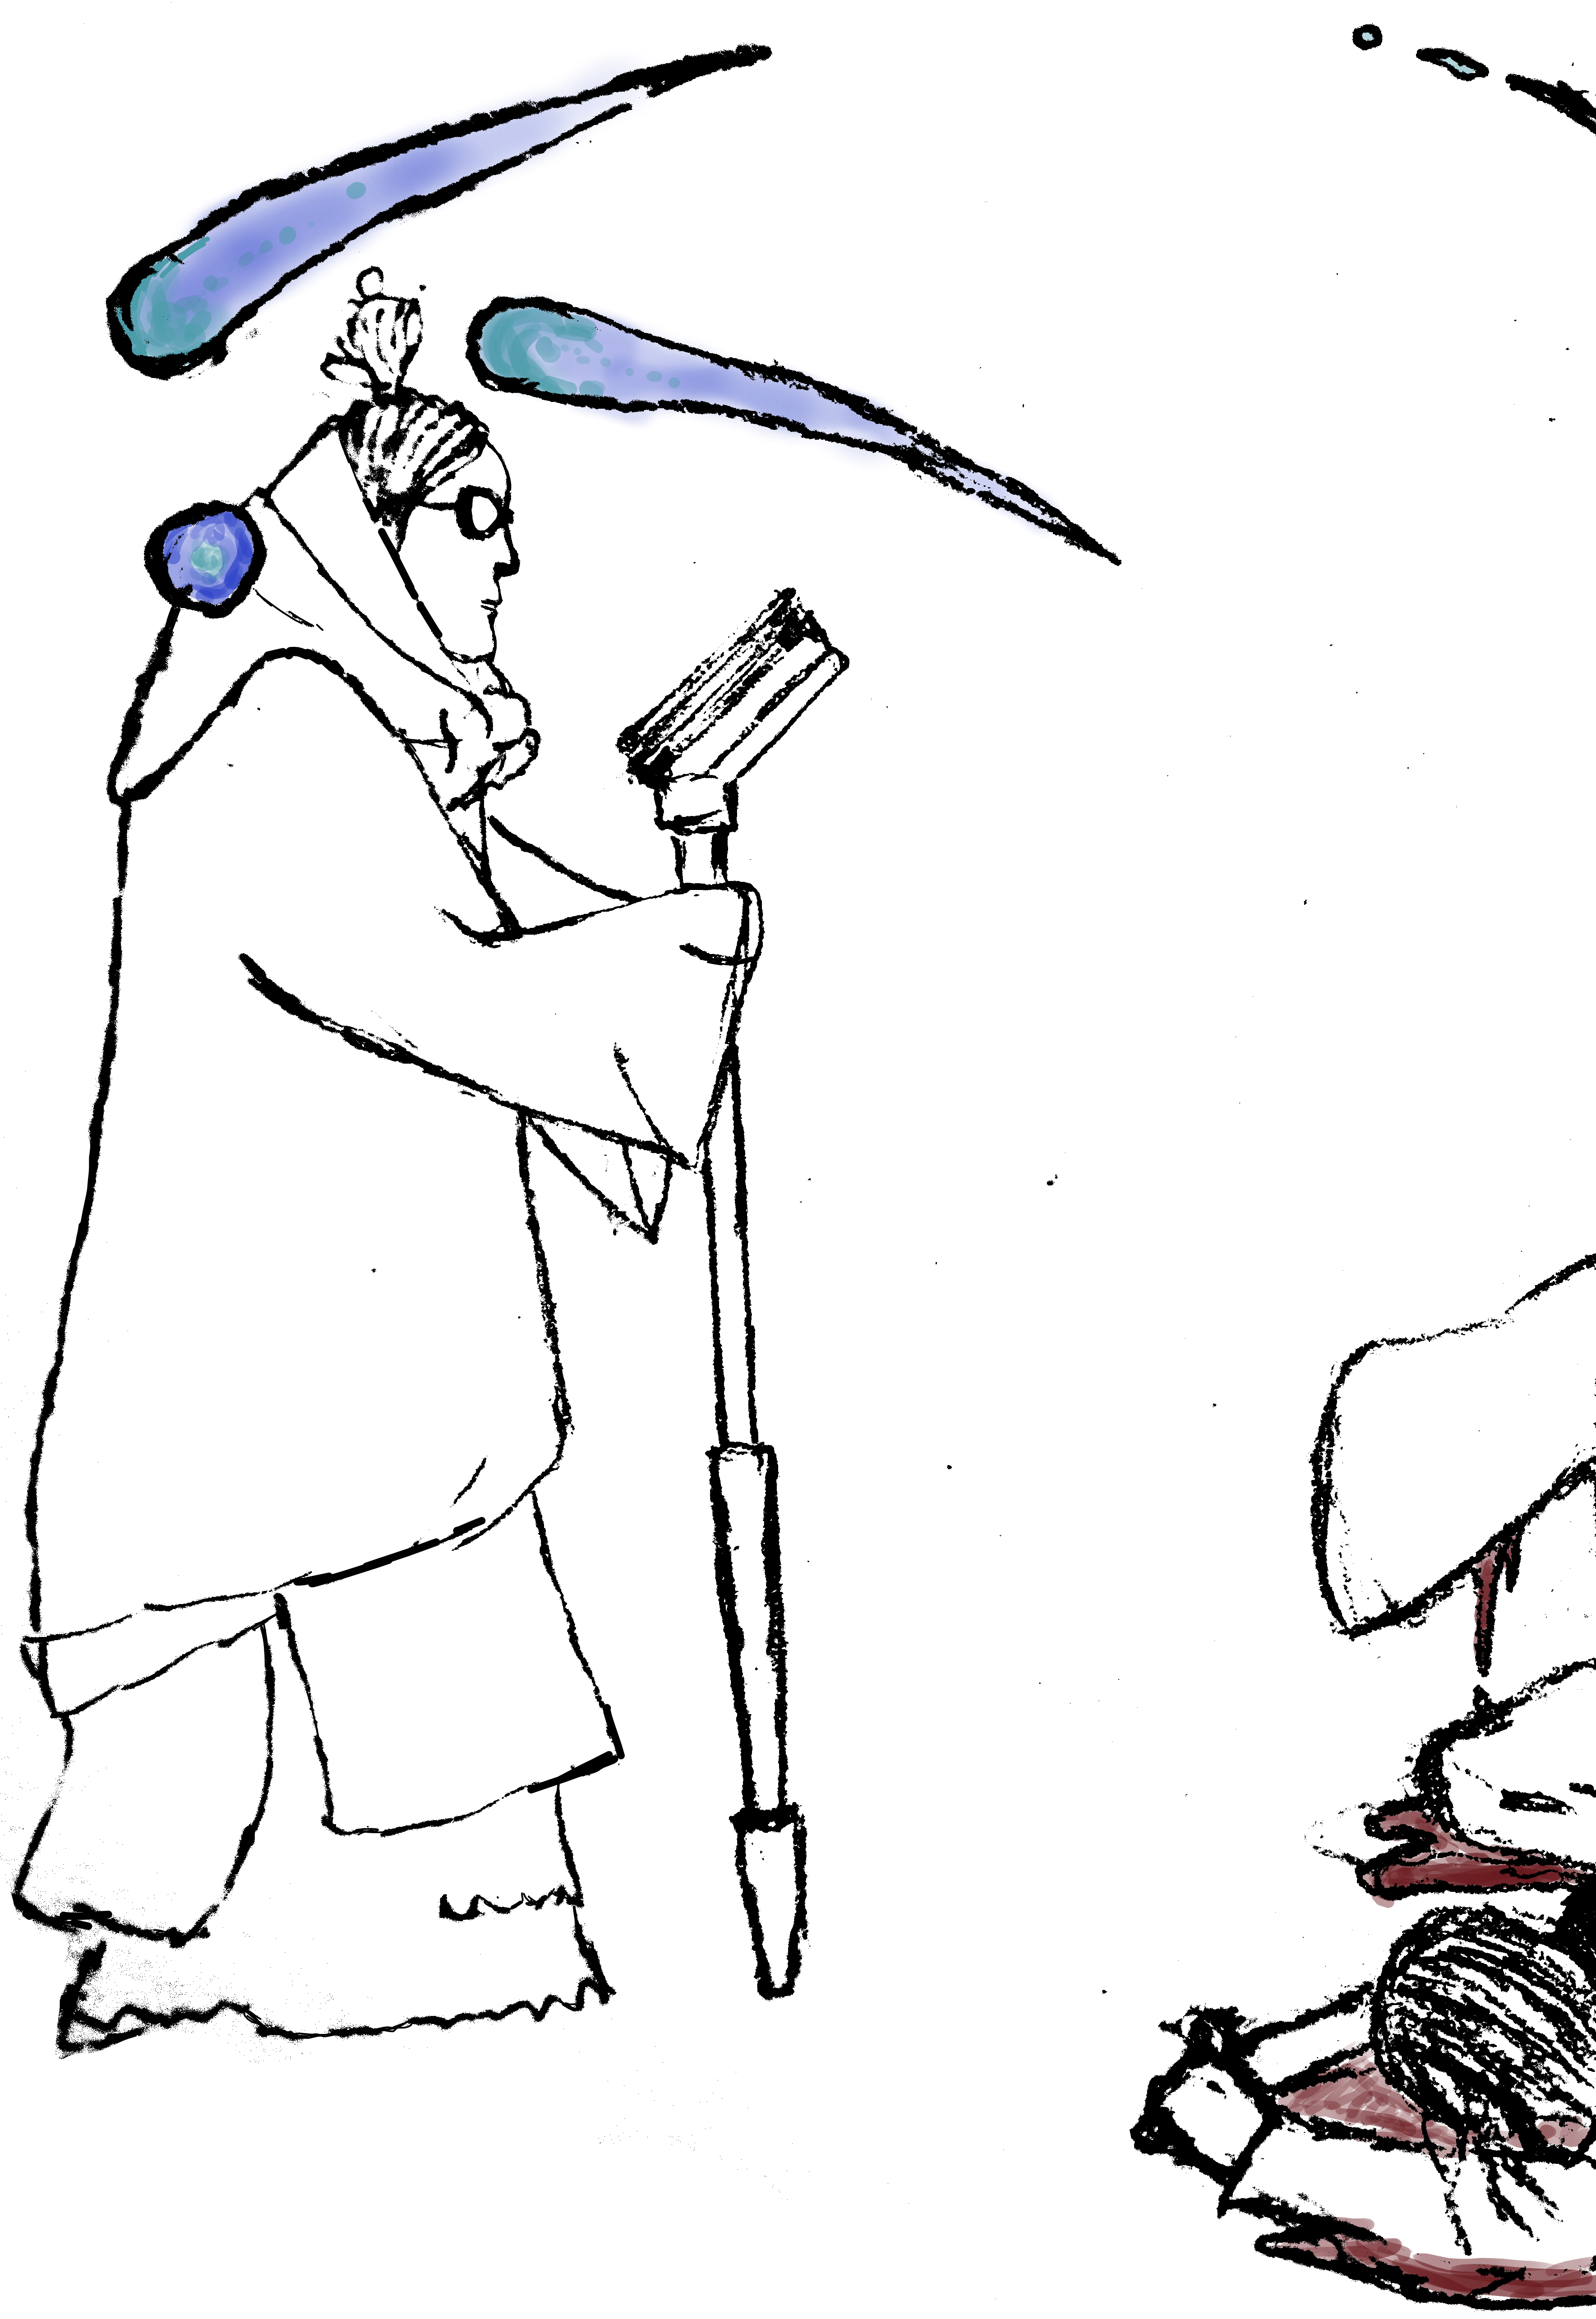
\includegraphics[width=0.5\paperwidth]{media/magic_missile_1-0.png}};

\begin{multicols*}{2}

\subsection*{Weaving a spell}

The power of a mage is represented by a \texttt{Spellweaving Pool}: a set of dice that you can use to weave spells. 

\colbox{
The spellweaving pool is described by

\begin{itemize}[nosep, leftmargin=*]
    \item Amount and kind of dice it can hold
    \item How one restores those dice
    \item What actions, if any, could change it
\end{itemize} 
}
If several effects grant you a spellweaving pool, those exist independently unless specified. Consuming \textbf{Spur} refills \texttt{3} dice from any combination of pools.

To weave a spell, a weaver rolls any number of those dice from any available pools as an Action from that set and then decides what to cast. This is a \texttt{Spellweaving roll}.
Only one spell can be cast per roll. If the spell does not state otherwise, \texttt{Smite} \texttt{Feat} is not applicable for attacks performed within them.

Each time after a spell is weaved in combat, caster needs to pass \texttt{Clarity Save} or become \texttt{Fatigued}. \textbf{No spell} can be cast until \texttt{Fatigue} is cleared.

There are many spells one can learn during their mage training, but regardless of syllabus -- all spellweavers know \textit{Detect Magic} by heart.

\newcolumn

\subsection*{Rethreading of the arcane}

When a mage rolls dice to weave a spell, in addition to casting, they can choose half, rounded down, of the remaining dice and discard the rest.
These chosen dice can be stored to cast spells later as if they are included in a roll.
They persist until spent, and count as in \texttt{Spellweaving Pool}. The amount of dice in the pool, both unused and stored, can't exceed its size.

% Several ways exist for how a person might become a mage. 
% A knight who has been taught spellweaving since childhood gets their \texttt{Spellweaving Pool} at character creation. 
% This pool is a set of \texttt{d6} dice with size equal to the value of their \texttt{Clarity}. 
% In order to restore dice, a knight must indulge their passion; this action restores \texttt{3} of them.


% \subsection*{Becoming a spellweaver}

% A knight who has been taught spellweaving gets their \texttt{Spellweaving Pool} at character creation. 
% They know any three spells from the list below in addition to \emph{Detect Magic} and one cantrip.
% \begin{itemize}[nosep, leftmargin=*]
%     \item \textbf{Dice} are all \texttt{d6}'s, and their amount is equal to the value of knights' \texttt{Clarity}.
%     \item \textbf{Restoring} the pool is done through \texttt{Overnight Rest} or indulging a \texttt{Passion}, both methods restore \texttt{3} of the missing dice.
%     \item \textbf{Improving} this pool is challenging; the limit of what could be thought is reached.
% \end{itemize}

\end{multicols*}


\newpage

\pagetopsection{ Creating a Spellweaver}


\begin{multicols*}{2}

\subsection*{Rolling stats}

\paragraph{Virtues.} Spellweaver's creation starts the same as one for a knight: roll \texttt{d6 + d12} four times; record not only the sum, but also individual values of each die, distribute them among \texttt{Virtues}, calculate \texttt{Focus} and \texttt{Stress}, determine \texttt{Injury slots}.

\paragraph{Guard.} Roll \texttt{d6} to determine the maximum \texttt{Guard(GD)} the spellweaver has.

\paragraph{Choose a Passion.} Indulging a Passion restores \texttt{Spirit} and \texttt{Spellweaving} dice (p.\pageref*{sec:spellweaving}), so choose it accordingly. That in large determines who your character is.

\paragraph{Feats.} Spellweaver knows no \texttt{Feats}. They are not trained to know marital secrets of hand-to-hand combat.

\newcolumn

\subsection*{Weapons \& Gear}

Spellcasters are not proficient with complex weapons or armour. 

Without additional training, spellweaver can't have more than one weapon dice per weapon they use(choose one if those are different), they also can't use armour plates.

\paragraph{Spellbook} is not only a way to store knowledge, but also a focal point of any spell you cast. If you hold it when weaving a spell you round up when calculating amount of dice you can store during \emph{rethreading of the arcane}. You can't hold it in the same hand you wielding a shield with.

\subsection*{Spellcasting}

It is assumed that you are either a very talented self-taught mage, went through formal training or a secret third thing to you tend to talk little about. 
Either way you are better at controlling the arcane then almost anybody else. 
That training is also source of your power.

\colbox{
\paragraph{Spellweaving pool}

\begin{itemize}[nosep, leftmargin=*]
    \item \textbf{Dice} are all \texttt{d6}'s, and their amount is equal to the value of weaver's \texttt{Clarity}.
    \item \textbf{Restoring} the pool is done through \texttt{Overnight Rest} or indulging a \texttt{Passion}, both methods restore \texttt{3} of the missing dice.
    \item \textbf{Improving} this pool is challenging; the limit of what could be thought is reached.
\end{itemize}

}

You know five spells(p.\pageref*{sec:spellweaving}) and one cantrip additionally to \emph{Detect Magic}.

\end{multicols*}


\newpage

\section*{\centering \fontsize{35}{45}\selectfont Familiar Arcana}
\vspace*{0.4 cm}

\begin{multicols*}{2}

\subsection*{Cantrips}

When casting a cantrip: pick one die, if its odd -- treat it as if you haven't cast the spell.

\paragraph{Light.} You create an immaterial sphere of pale blue light roughly the size of your eyeball. 
You can change the colour between reddish-yellow and bright blue. 
It lasts while you are conscious and no more than several step away. 
You can dismiss it at any time.

\paragraph{Wisper.} You whisper a message to the target you can see. 
They hear you as if inside their ear. 
They can whisper back to you as an answer. 
You can also whisper to somebody you know is there if you are separated by a non-magical wall less than a arm's reach thick.

\paragraph{Small Illusion.} You create a sound or an image of an object at location that you can see well.
If its an image -- it must be no larger than a 5-foot cube. If you create a sound, its volume can range from a whisper to a scream.

The illusion ends if you dismiss it or cast this spell again. 

\subsection*{Spells}

\paragraph*{Detect Magic.}

Pick any number of dice; for each one that rolled its maximum value, you can ask a question about surrounding magic and receive a truthful answer, but the number of words in that answer can't exceed the value rolled on the die.
For each other die, the answer is either yes, no, or silence if the question is not applicable.
Information for the answer is provided by yourself and spells around you.
For example, spells usually are not directly marked by their caster and are not aware of their surroundings beyond the spell's design.

\textbf{You can learn a new spell} unknown to you. 
Upon discovery, do a \texttt{Clarity} save; if successful, ask the Referee if you can learn this spell and, if you can, how many times encountering this spell in the wild is enough.

\paragraph{Soothing Visions. } Pick two dice both with the same value rolled as the target's \texttt{Stress}. 
Reduce their \texttt{Stress} by \texttt{2}.

\paragraph{Heat Metal.} Intricate ladder of arcane pulses rapidly heats metal until it glows red hot.
Pulses should be chained together carefully; pick no less than three dice with consecutive values.
If it is a piece of armour, the wearer takes \texttt{Damage} equal to the sum of chosen dice.
If it is a weapon, the bearer chooses to drop it or persevere through pain, taking half of the sum of the chosen dice.
Any \texttt{Damage} from this spell ignores \texttt{Guard}.


\paragraph{Hex.}
A curse of misfortune impairs defense and makes the target more vulnerable.
Pick three dice that have a value of \texttt{1}. Mark them as spent, but they can't go back to the pool while the spell lasts.

For the remaining combat, anyone who attacks the bearer of this curse can add a die from the picked ones as an additional weapon die before rolling.
The die is not spent and can be used by multiple attackers, but only a single Hex can be cast upon any one creature.
The spell is active for a couple of days or until dismissed. 

Outside of combat, any die can be used as a penalty to \texttt{Virtue} rolls that could be affected by luck, e.g., thoughts are generally unaffected, but physical and attention-dependent actions are.

\paragraph{Haste.} Pick any number of dice that amount to the target's Vigor or greater.
Each time a hasted creature attacks, choose a weapon and add its \texttt{Weapon dice} to the \texttt{Attack} one additional time.

\paragraph{True Strike.}
Pick any number of dice, then perform an Attack as usual.
You can replace any die of the attack with any die from those you picked.
Can be used with \texttt{Smite} \texttt{Feat}.

\paragraph{Shield.} Pick two dice and add the smaller rolled value among them to \texttt{Guard} of a willing creature nearby.
 The shield's \texttt{Guard} is spent before theirs.
 Shield's \texttt{Guard} persists until their \texttt{Guard} would be restored normally.

\paragraph{Magic missile.}
Identical glowing bolts launch towards chosen targets, piercing bone and muscle.
Pick any number of dice with the same value rolled.
You can pick a different target for each bolt; it deals \texttt{Damage} equal to the rolled value.

\end{multicols*}

\newpage

\begin{multicols*}{2}

\paragraph{Blade Ward.} Pick any number of dice -- they are locked into the spell until discarded.

Each time an attack would hit you for damage that is exactly equal to the value of any picked dice, treat the attack as if it was evaded. 
Return the matching die to the pool, it is no longer part of the spell. The spell persists until dismissed or all dice are spent.

\paragraph{Mind Sliver.} Pick any amount of dice, perform a ranged attack as if they are your weapon dice. 

However, the damage from this spell is dealt to \texttt{Spirit} or \texttt{Clarity} instead of \texttt{Vigor}. 
If half or more \texttt{Virtue} is lost as a result of this spell, the target's attacks are \texttt{Impaired} until your next turn.

\paragraph{Conjure embodiment of magic.} Pick up to two dice three times; values for each pick determine virtues of the embodiment.
Then pick an additional die -- this is its guard.
Embodiment obeys your commands and vanishes when any of its virtues reach zero.
At dawn of each day, you need to maintain it: pick up to two dice; that's the new Vigor of the embodiment.

Otherwise, halve each of its virtues, rounding down. Embodiments are unnatural for this world, so at dawn, reduce its Clarity by 2.
At the end of each combat, reduce its Spirit by 1.
You choose the shape and overall appearance of the embodiment, but it still looks very unnatural and magical for anybody who glances at it.

It has no armour, attacks for 2d8, and can use one \texttt{Feat} you choose each morning.
It is as intelligent as an orca, can't speak, but comprehends languages you know.
Does not really understand human ways, but can mimic them with mixed results.

\paragraph{Helping hands.} Pick any number of dice that amount to exactly ten. 
You summon a pair of hands to help you. 
You can control them directly or delegate simple tasks. Choose where they grow from; usually hips or shoulders are the best choice.
Your productivity increases greatly for tasks you already know how to perform. 

In combat, they can wield either \emph{two non-Hefty} weapons or \emph{one Hefty}. 
They are not very strong, so nothing heavier is feasible. You can still benefit from only one shield. 
They last for a task you summoned them to fulfill or for one combat. Slowly dissipate when idle.


\end{multicols*}

\newpage

\section*{\centering \fontsize{35}{45}\selectfont Witchcraft}
\vspace*{0.4 cm}

\label{sec:witchcraft}

\begin{multicols*}{2}

Witches cast spells as manifestations of favours granted to them by their patrons.
Favour is spent after a spell is complete and is regained when a witch indulges the passions of their patrons.

Cantrips don't cost favour, but stop working when a witch has none.

Each time after witch casts a spell in combat, they need to pass \texttt{Spirit Save} or become \texttt{Fatigued}. \textbf{No spell} can be cast until \texttt{Fatigue} is cleared.

\paragraph{Witch communes} with their patron at will as long as their favour is not zero.
Generally, a patron is helpful, but pursues their own goals and struggles to understand human ways outside of their domain. 
Favour determines how many times a witch can request an audience and expect an answer. 



\newcolumn

\subsection*{Uncovering a new spell} 

At first witch needs to convince the patron that they are ready by passing \texttt{Spirit} save. 

Witch loses amount of favour that is twice as much as the spell costs. It manifests as a small trinket which works as a puzzle, passing \texttt{Clarity} save is required to solve it.

After that, witch learns the new spell and can cast it as usual.


\end{multicols*}



\newpage

\pagetopsection{ Creating a Witch}


\begin{multicols*}{2}

% TODO: invocations instead of spells

\subsection*{Rolling stats}

\paragraph{Virtues.} Creation of a witch starts the same as one for a knight and a spellweaver: roll \texttt{d6 + d12} four times; record not only the sum, but also individual values of each die, distribute them among \texttt{Virtues}, calculate \texttt{Focus} and \texttt{Stress}, determine \texttt{Injury slots}.

\paragraph{Guard.} Roll \texttt{d6} to determine the maximum \texttt{Guard(GD)} that witch has.

\paragraph{Choose a Passion. } Indulging a Passion restores \texttt{Spirit}, so choose it accordingly. 
That in large determines who what your witch actually draws their strength from.

\paragraph{Feats. } Witch knows no \texttt{Feats}. They had no access to martial art training or chose not to participate.

\newcolumn

\subsection*{Weapons \& Gear}

Without additional training, witches can't have more than one weapon dice per weapon they use(choose one if those are different), they also can't use armour plates.

\subsection*{Spellcasting}

Witch casts spells by invoking power of their patron. 
This is mutually beneficial agreement, patron expects for a witch to act on their behalf in the world of mortals.

Witch start with \texttt{2d4} favour and replenishes it by indulging patron's passions. 
At the start a witch knows 5 spells of their patron and all cantrips. 

\end{multicols*}


\newpage

\section*{\centering \fontsize{35}{45}\selectfont Thaliat, the laughing spirit}
\vspace*{0.4 cm}

\begin{multicols*}{2}

Thaliat's passion is of laughter, festivals, and theater.
She craves stories and tales.
Enjoys performances that are done out of pure heart.
Treasures celebrations that bring sincere joy for those who participate.

\paragraph{Cantrips}
\begin{itemize}[nosep, leftmargin=*]
    \item[\ding{108}] \textbf{Prestidigitation}, a nothing spell. Sparkles, small lights, whispering sounds, change of colour.
 The more inconsequential something is, the more probable it is a shape of Prestidigitation.
    \item[\ding{108}] \textbf{Mending}, a minor repair spell. Fixes a tear in fabric, crack in leather, or a snapped thread.
\end{itemize}

\paragraph{1 Favour spells}
\begin{itemize}[nosep, leftmargin=*]
    \item[\ding{108}] \textbf{Last call bell.} You start a dance, a trick, or any other performance. As long as you are doing it, all doors to the room you are in, except maybe one, close and lock themselves.
    \item[\ding{108}] \textbf{Curtain drop.} You bow down as if you just ended a performance. Smoke or water mist envelopes you for a few seconds, giving you and up to one other person near you an opportunity to escape combat.
    \item[\ding{108}] \textbf{Invisible helper.} You summon an invisible, almost immaterial creature that obeys your mental commands. It can move and carry objects that a determined child can; it is easily scared of violence and likes sweets. Disappears when you fall unconscious.
    \item[\ding{108}] \textbf{Failed Rehearsal.} When you fail a \texttt{Spirit Save} or \texttt{Clarity Save}, you can immediately retry it. Each save can benefit from this spell only once.
    \item[\ding{108}] \textbf{Disguise Voice.} Make your voice appear as somebody else's whom you heard within at least one conversation.
\end{itemize}
\paragraph{2 Favour spells}
\begin{itemize}[nosep, leftmargin=*]
    \item[\ding{108}] \textbf{Am I here, am I there.} Suddenly it is very hard to understand where you are and what you are doing.
 Anybody who looks at you feels confused and puzzled, unable to understand your intentions.
 In combat, it means that for the remainder of it, when you \texttt{Deny} -- an additional die of your choice is discarded.
    \item[\ding{108}] \textbf{Cursed Joke.} You tell your vilest joke and sprinkle enough magic to take it inside the target's head. Upon hearing it, target retracts themself from any conversation they were having or any activity they were doing.
 Goes to the corner or seeks solitude if the corner is unavailable and sits there in an increasingly catatonic state. The target falls unconscious after 10 minutes; when woken up, the effect ends.
 Their memory preserves a feeling of unpleasantness, but the content of the joke vanishes.
 If the target is in combat, their \texttt{Attacks} are \texttt{Impaired} until the effect ends.
\end{itemize}
\paragraph{3 Favour spells}
\begin{itemize}[nosep, leftmargin=*]
    \item[\ding{108}] \textbf{Let me try one more time.} When you fail a \texttt{Save} targeted by \textit{Failed Rehearsal}, you can retry one more time.
    \item[\ding{108}] \textbf{All doors are open for me.} Opens any non-magically locked door
    \item[\ding{108}] \textbf{You are an actor too.} For an hour or until harmed, the target thinks that they are somebody else \textbf{they} have a strong impression of.
 The target acts according to their own understanding of that entity.
 Upon recovery, they remember vaguely what happened during the effect of this spell.
\end{itemize}

\end{multicols*}


\newpage

\pagetopsection{ Vesna, the passage guardian}


\begin{multicols*}{2}

Deep forest is her domain, where she guards gates between our world and the world of the dead.
She seeks to guide those who are stuck in between.
Gives her blessings if one helps a scared soul to complete their journey.
Cares for both people and animals alike.
Despises cruelty and sometimes plays with children, who can still see her.
Knows about improper burials and rewards those who make peace with the dead.


\paragraph{Cantrips}
\begin{itemize}[nosep, leftmargin=*]
    \item[\ding{108}] You travel through forests as fast as a horse rider would travel on a road.
    \item[\ding{108}] \textbf{I help, you provide} You sense local distress of the wilderness.
 When you resolve it, you can ask for something in return.
 If it could be found here, it's gonna be provided to you.
\end{itemize}

\paragraph{1 Favour Spells.}

\begin{itemize}[nosep, leftmargin=*]
    \item[\ding{108}] \textbf{Be not afraid.} Talk with animals: they understand you; you understand them.
    \item[\ding{108}] \textbf{Tell me your story.} Talk with the dead, provided you have something they owned
    \item[\ding{108}] \textbf{Forest, obscure me.} As long as there is enough foliage around, it shifts to provide cover, making you and maybe one of those with you almost impossible to find.
    \item[\ding{108}] \textbf{I've never said that I am done. } You move fast, and your weapon moves almost on its own. For the remainder of the combat, each time you \texttt{Attack}, you can do an additional \texttt{Gambit} without expending a die.
    \item[\ding{108}] \textbf{Vesna guides you. } Choose a willing creature; next time they attempt a roll with at least \texttt{1} \texttt{Focus} -- they roll as if an additional \texttt{Focus} was spent.
\end{itemize}

\paragraph{2 Favour Spells.}

\begin{itemize}[nosep, leftmargin=*]
    
    \item[\ding{108}] \textbf{Grow my beloved, grow.} You put a new life into potentially dead vegetation with your touch.
 It grows very fast and obeys your commands.
 Branches can grapple your enemies, fix objects, and obstruct passage.
 Without water and soil, it dies soon after you leave, expending all its resources.
 For example, it takes 10 minutes to make a wooden door frame impassable, but only several seconds to make a wooden door impossible to open.
 In combat, it immobilizes enemies on the round of casting and impairs weapons until escape(\texttt{Vigor Save}) on later turns.
    \item[\ding{108}] \textbf{It hurts, I know.} Transfer a \texttt{Trauma} from one willing creature to another willing creature of roughly the same consciousness level.
    \item[] \item[\ding{108}] \textbf{They are within reach.} When you search for somebody you know, you can determine if this person is dead or alive and peek into their thoughts and emotions.
\end{itemize}

\paragraph{3 Favour Spells.}

\begin{itemize}[nosep, leftmargin=*]
    \item[\ding{108}] \textbf{There is only a single path.} When you go through a door, you envision another door that you have traversed in the past day by non-magical means.
    As long as you hold the door open, it leads to the place the door you envisioned leads to. 
    \item[\ding{108}] \textbf{Look, we are alike.} You touch a willing animal and assume some of its traits: talons, fins, teeth, fur, etc. You choose what suits you best.
 You can share these traits with somebody if you keep physical skin contact with them for the whole time.
 Effect lasts until dismissed.
    \item[\ding{108}] \textbf{Let me take all the pain.} You touch a willing creature and transfer any one of their \texttt{Injuries} to yourself.
\end{itemize}

\paragraph{4 Favour Spells.}

\begin{itemize}[nosep, leftmargin=*]
    \item[\ding{108}] \textbf{You and me: friends.} You summon an animal to aid you. 
    It understands you when you speak with it, can't speak back, but can transmit emotions and follow simple instructions. 
    You can choose any size as long as it is no larger than a well-fed barn cat. 
    Depending on the size, roll for \texttt{Vigor}. Roll 1d1 if it's tiny, like a mouse; 1d4 for a bird, like an owl; 2d4 for a badger or opossum; d8 for a cat or a small dog. 
    Roll d6 for \texttt{Clarity} and \texttt{Spirit}. Roll d4 for \texttt{Guard}. If it dies, you can summon it again after sunset. 
    Its natural weapons allow it to attack for a \texttt{d4} damage. It can perform \emph{Bolster}, \emph{Impair}, \emph{Move} and \emph{Stop} gambits.
    It has one \texttt{Severe} injury slot.
\end{itemize}

\end{multicols*}


\newpage

\section*{\centering \fontsize{35}{45}\selectfont Aestur, the ravaging spirit}
\vspace*{0.4 cm}

\begin{multicols*}{2}

In the beginning there were stillness and staleness. The sky and the earth were solid and flat and iron. The light didn't travel through space but was preserved frozen in one place, and nothing was seen or heard, and nobody was looking and listening. The cosmos got bored of itself.

But even in constant there is a change. A curious atom came into being under the iron sky. It ran and played along the iron folds and collided and fell and gained velocity until the iron started to ring and sing.

And there was a great ramble and great fire. The iron earth collided with the iron sky. Aestus, the ravaging spirit, was born. The havoc ensorcelled it, and Aestus became determined to destroy. With great power, it broke off a mace out of the iron plane and went on a rampage through the universe.

And there were many things born in destruction. Light and sound, sand and water, fire and stars were the sparks of the great rumble. They were destroyed by Aestus in their turn.

But nothing was sufficient to satiate the ravaging spirit. He took a handful of dirt and made beasts, fish and people, who suffered being tossed and crushed.

By now we live, but soon comes the day we perish under the iron mace of the Aestur. No will be spared.

Each time you roll maximum on your weapon die and chose it as a damage die of your attack, gain one favour for each point of damage which reduced targets \texttt{Vigor}.

\paragraph{Cantrips}
\begin{itemize}[nosep, leftmargin=*]
    \item[\ding{108}] \textbf{No, you can't have that.} You crush a small non-living object just outside of your reach. The force you impose is enough to snap anything you can snap with your one hand.
    \item[\ding{108}] Any time you would attack while having one hand free of the weapon. You can summon a Mace of Aestur for the attack. It's a \textbf{Hefty} d8 weapon. 
    You can spend any amount of favour, upface the Mace's weapon die for each spent.
\end{itemize}

\newcolumn{}


\paragraph{1 Favour Spell}
\begin{itemize}
    \item [\ding{108}] \textbf{Let this iron eat your flesh.} From a piece of iron you touch splits a rough, razor-sharp splinter with jagged edges. You fling it for \texttt{d6 damage}. 
    If you rolled \textbf{6} on this damage die, you can discard it. In that case you choose either: to mortally wound(p.\pageref*{sec:hopefear}) your victim or deliver one \texttt{Severe Injury} or execute one Strong Gambit. 
    \item [\ding{108}] \textbf{Remember your weakness.} Let the presence of Aestur poss you for a split second to project power and induce fear. 
    That intimidates those near you. Treat the \texttt{Spirit} roll target makes to resist as if it is opposed with \texttt{1} additional \texttt{Stress}. 
    In combat, treat next incoming attack as if you allocated an additional \texttt{Focus} to your \emph{Defense}(p.\pageref*{sec:basic}) for each attacker.
\end{itemize}

\paragraph{2 Favour Spell}
\begin{itemize}
    % \item [\ding{108}] \textbf{Hear me.} You clap your hands with deafening clang of metal. This is a melee attack with \texttt{d4 Blast} damage dice.
    % Those in immediate vicinity of you who did not expect that do \texttt{Spirit} save and have their attacks impaired until your next turn if failed. The sound can be heard from \textbf{very} far.
    \item [\ding{108}] \textbf{This is mine now.} Turn a non-living palm-sized object you touch into solid pure iron. 
    Fine details can't be preserved, e.g. lock will stop working if you alter it like that, but cracks and imperfections vanish. 
    If you throw this object as a ranged attack it has \texttt{2d4} weapon dice. 
    \item [\ding{108}] \textbf{Rage flows through me.} Until the end of combat you can reroll any weapon dice which rolled \texttt{1} on it. You must use the new value rolled.
\end{itemize}


\paragraph{3 Favour Spell}
\begin{itemize}
    \item [\ding{108}] \textbf{Your staff is broken.} Crush a non-living object you can clearly see. Enough to destroy wooden shields and weapon handles. 
    Not enough to destroy bricks and stone, but enough to send their shrapnel flying with \texttt{2d4 Blast} weapon dice originating from the object.

    
    
\end{itemize}


\end{multicols*}


\newpage

\pagetopsection{ Corrust, the spirit of dwindling}


\begin{multicols*}{2}

\

\end{multicols*}

\newpage

\section*{\centering \fontsize{35}{45}\selectfont Quirks}
\vspace*{0.4 cm}

\label{sec:quirks}

\begin{multicols*}{2}

\paragraph{Bloodlust.} A visceral reaction to blood fuels strength, but lessens control.
You can \texttt{Upface} one die of your weapon if you are \texttt{Wounded}(p.\pageref*{sec:wounded}). However, if somebody is wounded, you can't engage them with nonlethal force.

\paragraph{Desensitized.} The things you saw made everything else bleak in comparison; you don't feel much ever since.
When you treat an injury on the battlefield, you roll with an additional \texttt{Focus}. However, you can't treat yourself.

\paragraph{Thick-skinned.} After you recover, your skin changes. It became rougher and harder to pierce.
You ignore the first \texttt{Damage} to your \texttt{Vigor} per combat if it is not larger than \texttt{2}.
However, when your injury is treated on the battlefield, the roll is treated as if it is opposed with an additional \texttt{Focus}.

\paragraph{High pain tolerance.} Your body seems determined to never let you suffer again.
You can ignore up to one \texttt{Agony} consequence of your \texttt{injury}.
However, each time you roll a 20 on a \texttt{Vigor Save}, you lose \texttt{1} \texttt{Vigor}.

\paragraph{Masochistic.} Pain is unbearable, but somehow it's a good thing. You regain all \texttt{Focus} each time you suffer an \texttt{Injury}.
However, don't recover \texttt{Focus} during \texttt{Short Rest}.

\paragraph{Blade obsession.} At the beginning of each day, randomly determine a weapon you own that you are obsessed with.
You can \texttt{Upface} any die of that weapon. However, each time you strike, you must strike with the weapon you are obsessed with.
You can't part with it; during combat it must be in your hand, otherwise at arms length at most.

\paragraph{Gore fascination.} You ignore \texttt{Distress} afflictions of your \texttt{Injuries}.
However, you must treat your \texttt{Injuries} by yourself.

\paragraph{Stressjunkie.} Each time you gain \texttt{Stress}, also gain \texttt{Focus}.
However, your maximum \texttt{Stress} is halved, rounded up. It can't go lower than \texttt{1}.

\paragraph{Sadistic.} Restore one \texttt{Focus} each time an \texttt{Attack} you participate in reduces both \texttt{Vigor} and \texttt{Guard}.
However, gain one \texttt{Stress} when an attack you participate in does not reduce the target's \texttt{Vigor}. If this point of \texttt{Stress} would cause \texttt{Trauma}, gain no \texttt{Stress} instead.

\paragraph{Smile like no other.} You don't smile a lot, but when you do, people feel what you have been through.
You can \texttt{Downface} any die that is used in an Attack against you.
However, whenever you take a \texttt{Clarity} save during socialization, treat it as if it was opposed with one additional \texttt{Focus}.

\paragraph{Traumatic visions.} Each time you swing at your enemy, pain returns. You can keep it at bay, but it takes effort and willpower you don't always have to spare.
Each time you roll with \texttt{Focus}, you can \texttt{Upface} one die before choosing what die to copy. 
However, each time you roll without \texttt{Focus} -- \texttt{Downface} one die in your roll.

\paragraph{Overconfident.} For some reason, after all the pain, you feel like you have figured it all out. Each time you perform a \texttt{Feat} -- gain one \texttt{Focus} after the attack. 
However, each time you are \texttt{Fatigued} -- lose \texttt{2} \texttt{Spirit}.

\paragraph{You never learned.} Record each time you are \texttt{Fatigued}. Each third time, reset the count, resist the \texttt{Fatigue} and gain \texttt{2} \texttt{Stress}.

\paragraph{Strength in suffering.} When you attack, upface a die if you have at least one \texttt{Injury Slot} filled with active \texttt{Affliction}.

\paragraph{Food aversion.} You suffer when eating food that is not cooked by you. 
During overnight sleep you restore a single point of virtue if you are not the one who cooked the meal.
However, if you cooked it yourself -- the Company, including you, restores and additional point of virtue instead.



\end{multicols*}


\newpage

\section*{\centering \fontsize{35}{45}\selectfont Traits}
\vspace*{0.4 cm}

\label{sec:traits}

\begin{multicols*}{2}

\subsection*{Paths unfinished}

\paragraph{Abandoning squireship} was not an easy decision, but not every squire destined to become a knight. 
However, that does not mean all this time is wasted: you leaned a lot during those years. 

You know one \texttt{Feat} of your choice. You also know how to deal with armour plates and complicated weapons.

\paragraph{Unacknowledged presense} in your dreams calls you. In times of struggle, you learned that you can ask it for help in exchange for a promise. 

Choose a patron: you know what they want and can use \texttt{2} of their spells.
You can learn more the same way as a witch(p.\pageref*{sec:witchcraft}) does.
    
\paragraph{Lurking spellweaving} followed you around all your life, but either mages you encountered did not recognise the potential, you avoided training following your own reasoning or you were taught by a very conservative curriculum.

\colbox{

\begin{itemize}[nosep, leftmargin=*]
    \item \textbf{Dice} are all \texttt{d6}'s and there 3 of them
    \item \textbf{Restoring} the pool is done through \texttt{Overnight Rest} or indulging a \texttt{Passion}, both methods restore \texttt{3} of the missing dice.
    \item \textbf{Improving} this pool is done by learning new spells: each time you succeed in that add an additional \texttt{d6} to it, up to half of your \texttt{Clariy} rounded down in total.
\end{itemize}
}

You know one cantrip and one spell in addition to \emph{Detect Magic}. 


\subsection*{Martial traits}

    % TODO: some flavour text about trading spellcasting for combat prowess.

\paragraph{Fluency of Combat} occasionally comes to those who never engaged with the world of magic.

During fights, you can spend your \texttt{Guard} to move in a strange dance of blade and fury. 
When deciding what dice to spend on Gambits, you can use dice with value below \texttt{4} as long as you compensate the difference by reducing your \texttt{Guard}.

\newcolumn

\paragraph{Weapon mastery} manifests when a knight develops an uncanny fascination with their weapons. 
They treat them not as mere tools of the craft, but as partners or trustworthy friends.

That allows them to see beyond the material, beyond the function, but towards possibilities.

Each time you roll a maximum value on a weapon die, put a mark on the weapon it belongs to. 
When amount of marks matches its largest weapon die -- you obtain a level of mastery with this weapon. 

When you use \texttt{Focus} or \texttt{Stress} and choose to duplicate the dice that belong to your weapon -- for each mastery level
you can keep the dice that otherwise would be discarded due to accumulated \texttt{Advantages}.

Weapon mastery levels do not transfer between any weapons even if they are of the same type, e.g. replacing one shortsword with another does not allow to keep the mastery level.

% \paragraph{Riposte} is a risky and potentially deadly \texttt{Feat}. If you choose to \emph{Riposte}, you can use it instead of \texttt{Deny Feat}. 
% Roll your weapon dice as if you are performing an attack. 
% Spend any amount of \texttt{Hope} or \texttt{Focus} you allocated for \emph{Defense}, keep one weapon dice per point spent.
% % Choose the number of them equal to \texttt{Focus} you allocated to \emph{Defense}, spending one point per dice. You can also spend Hope to add those dice.

% You can match any of your dice with lower dice in the attack roll against you. 
% Deal damage equal to the sum of pairwise differences between matched dice. Discard enemy's dice that were matched. 
% The damage of the enemy's attack after \emph{Riposte} ignores your \texttt{Guard}.

% Pass a \texttt{Spirit} save or become \texttt{Fatigued}.

\subsection*{Arcane traits}

\paragraph{Rethreading dominion} permits a whole new level of control over spellweaving threads.

When choosing dice to store during \emph{rethreading the arcane} you can combine those dice instead of storing them individually according to steps below.

\colbox{
\begin{enumerate}[nosep, leftmargin=*]
    \item Identify dice to combine among the dice chosen for rethreading
    \item Mark one of them as accumulation die
    \item Add all values among identified dice and set the accumulation die to that value
\end{enumerate}
If the accumulation die can't hold that value -- \emph{rethreading of the arcane} fails.
}

For example, if you chose to store two \texttt{d6}'s with values \texttt{2} and \texttt{3} you can instead store them as a single \texttt{d6} with a value \texttt{5} on it. 

On the other hand if you choose to store two \texttt{d4}'s with the same values rethreading fails as \texttt{d4} can't store value of \texttt{5}. 
If one of them is \texttt{d6} instead, it becomes possible again.

% \subsection*{Wiccan traits}

% \paragraph{Natural affiliation} blooms when witch and their patron have personal synergy that permits them to reach understanding of each other no other can achieve.

% TODO: hmm, patron polycule, no tax on learning spells?

\end{multicols*}


\newpage

\section*{\centering \fontsize{35}{45}\selectfont Sickness \& Malady}
\vspace*{0.4 cm}

\begin{multicols*}{2}

\subsection*{Venomous Snakebite}

There is no antivenom. The only way to survive is to ask a mage for a concoction.
They will provide it, but the treatment warps the body to assume enough features for poison resistance to take hold.
Those changes are irreversible.

Your pupils might turn vertical, scale to appear in places where new skin would have grown.

One can find additions to internal mouth structure or lower back growths.

\begin{itemize}[nosep, leftmargin=*]
    \item Once per combat, you spit venom out of your mouth. It is quick and unexpected: add a \texttt{d8} to your weapon dice.
    \item Shape of your head slightly changes, so you can't wear rigid headwear if its not custom made for you.
\end{itemize}


\subsection*{Mocking Sickness}

Once, when wounded, you witness that there is no flesh and no blood inside you.

In its place you find only crumbling clay, withered fabric, and sawdust.
However, despite all the differences, you feel the same. Maybe a bit duller to the touch and less pain.
At last, you notice that your wounds are not healing.

\begin{itemize}[nosep, leftmargin=*]
    \item You don't lose Vigor. Since you discover this change in yourself, record \texttt{Damage} you receive that would have been subtracted from your \texttt{Vigor}.
    \item For each 3 points of \texttt{Damage} accumulated this way treat your maximum \texttt{Vigor} as if it is reduced by \texttt{1}. When it reaches \texttt{0}, your body loses structural integrity and dissolves to dust.
    \item You accumulate \texttt{Injuries} based on \texttt{Damage} received and wither away when you are out of \texttt{Injury slots}.
    \item You can kinda feel how your insides should be arranged and don't feel much pain, so you can mend yourself from two \texttt{Injuries} during one \texttt{Long Rest} without rolls.
\end{itemize}
If you find a puppet master that will agree to such an outstanding demand, they could try to patch your body to restore its former shape, reducing the recorded \texttt{Damage}.

\subsection*{Bloating Infection}

Your wound is infected, and at some point in your fever-induced delirium you met a foreign presence.
It asked you to receive a gift.

The fever was gone in a day. Your recovery amazed anybody who has ever seen an infected wound like yours.

You feel the tint of that presence in each movement of your limbs, in each twitch of a muscle, in each breath and sip of water.
Numbness, slowness, swelling of legs and arms. Your skin never recovered its natural colour; your chest and stomach bloat, your breathing becomes sluggish, with unsettling rocking in your lungs.

You move with visible delay, and your reaction is impaired.
When injured -- you feel neither pain nor distress.

\begin{itemize}[nosep, leftmargin=*]
    \item Each time you do \texttt{Overnight Rest} if your \texttt{max GD} is greater than \texttt{1} reduce it by \texttt{2}.
    \item For each \texttt{2} \texttt{Guard} lost this way increase your maximum \texttt{Vigor} by \texttt{1}, up to \texttt{19}.
    \item You ignore \texttt{Afflictions} of \texttt{Injuries}.
\end{itemize}

\subsection*{Weavering Parasite}

Parasite awakes and digs into your body.
You feel a flash of agony, and then it's gone. Unnatural motions of muscles and skin are the only evidence of where it is.
In a day, it reaches your brain and hatches. You can sense more of the arcane than ever before: learn the \textit{Detect Magic} spell.

However, thoughts become murky, and your mind drowns in fog. 
You lose \texttt{1} \textit{maximum} \texttt{Clarity} and now have a \texttt{Spellweaving Pool} with a size of \texttt{1} filled with a single \texttt{d4}.

\begin{itemize}[nosep, leftmargin=*]
    \item Each morning you must feed the parasite.
    After waking up, roll a die from your \texttt{Spellweaving Pool}, lose that much \texttt{Clarity}.
    Restore \texttt{1} spent die from the pool.
    \item Record total amount of \texttt{Clarity} lost this way.
    For each \texttt{5} \texttt{Clarity} lost -- lose \texttt{1} \textit{maximum} \texttt{Clarity}, increase pool size by \texttt{1} and add an additional \texttt{d4} to the pool.
    Permanently \texttt{Upface} it once for each other die in the pool.
    \item When you have a \texttt{d12} added this way -- parasite is fully matured and stops feeding.

\end{itemize}

\end{multicols*}


\newpage

\begin{multicols*}{2}

    \subsection*{Detached Soul}

    When your body takes critical damage, instead of succumbing to injuries and pain, your soul detaches and continues to fight.

    \begin{itemize}[nosep, leftmargin=*]
        \item When you can't allocate a new \texttt{Injury}, you don't die. Instead, your body collapses, and your ghostly form emerges.
        \item It has \texttt{1} \texttt{Vigor}, \texttt{0} Armour, but otherwise keeps your parameters.
              Physical \texttt{Damage} applies to you the same, but targets \texttt{Spirit} instead of \texttt{Vigor} and ignores armour.
        \item You keep your \texttt{Traumas}, but not \texttt{Injuries}. For damage to \texttt{Spirit}, do the same \texttt{Injury} calculations as for \texttt{Vigor}, but receive \texttt{Trauma} instead. If you can't fit a new \texttt{Trauma} -- you are \textbf{Slain}.
        \item You can't be grappled, pushed, or moved, and you can't do the same to interact with objects. So, you can't perform \texttt{Gambits} that require physical interaction. However, you can \texttt{Bolster} just fine.
        \item You deal \texttt{damage} to \texttt{Spirit} and you can give \texttt{Trauma} if you would have dealt enough damage to cause an \texttt{Injury}. Additionally, ignore armour for \texttt{Injury} and \texttt{damage} calculations.
        \item You can't use \texttt{Deny} \texttt{Feat}, but gain ability to go through physical objects.
              There is no limit, but when there is no light, you can lose sense of direction and become trapped.
        \item If your physical body dies -- you persist, but it's easier to return to your own mortal vessel than to find a new one. There are no obvious ways to do either, though.
    \end{itemize}
You can choose the appearance of your soul and keep two pieces of your gear and one weapon.

    \subsection*{Particular Brain Damage}

    There was a lucky sword strike or a very violent night out. After waking up, you realise that the world is different from what you remember. 
    Learn the \textit{Detect Magic} spell.

    You gain a \texttt{Spellweaving Pool} with two \texttt{d4} in it. 
    Each time you reach maximum \texttt{Clarity}, roll the maximum die in your \texttt{Spellweaving Pool} and lose that much \texttt{Clarity}. 
    You may permanently \texttt{Upface} one die in your \texttt{Spellweaving Pool}. 

    \newcolumn

    \subsection*{Split Personality}

    Your mind overloads with stress; you feel like insanity approaches, but instead of collapsing into the abyss -- your consciousness splits, and now you are not just one, but two.

    You create another knight that from now on inhabits your body. 

    \begin{itemize}[nosep, leftmargin=*]
        \item Roll three \texttt{d12 + d6} and pick two of them and assign to \texttt{Clarity} and \texttt{Spirit}. Determine values of \texttt{Focus} and \texttt{Stress} for your new personality and track these separately from the old ones.
        \item Decide if they are a \texttt{Spellweaver}, a \texttt{Witch} or neither.
        \item Both of you still share \texttt{Vigor}, \texttt{Injury Slots} with their contents and \texttt{Guard}.
        \item Both of you acquire \texttt{Quirks} independently, share corporal illnesses, and must switch upon gaining \texttt{Trauma}, which is shared between the two of you.
        \item You can willingly switch governing personality by acquiring \texttt{1} \texttt{Stress}.
        \item Pick their \texttt{Passion} and, finally, a name. 
    \end{itemize}
Once the splitting event occurs, you switch to the new personality immediately. 


    \subsection*{Unsettling Discovery}

    You can't refill any \texttt{Spellweaving pool} by resting or indulging a passion. If you didn't have a \texttt{Spellweaving pool} before, you get one. 

    Each time you receive damage, record the damage die. \textbf{Upface} it for each time it was \texttt{Bolstered}. \textbf{Downface} it for each point of damage which was reduced by \texttt{Armour} or did reduce \texttt{Guard} instead of \texttt{Vigor}.

    Add this die to any of your \texttt{Spellweaving pools}. You add this die even if your pool is full. 

    Learn the \emph{Detect Magic} spell.

\end{multicols*}


\newpage

\input{sections/23-Forgotten-spells.tex}

\newpage

\input{sections/24-Forgotten-spells.tex}


\newpage
\label{sec:ch_sheet}
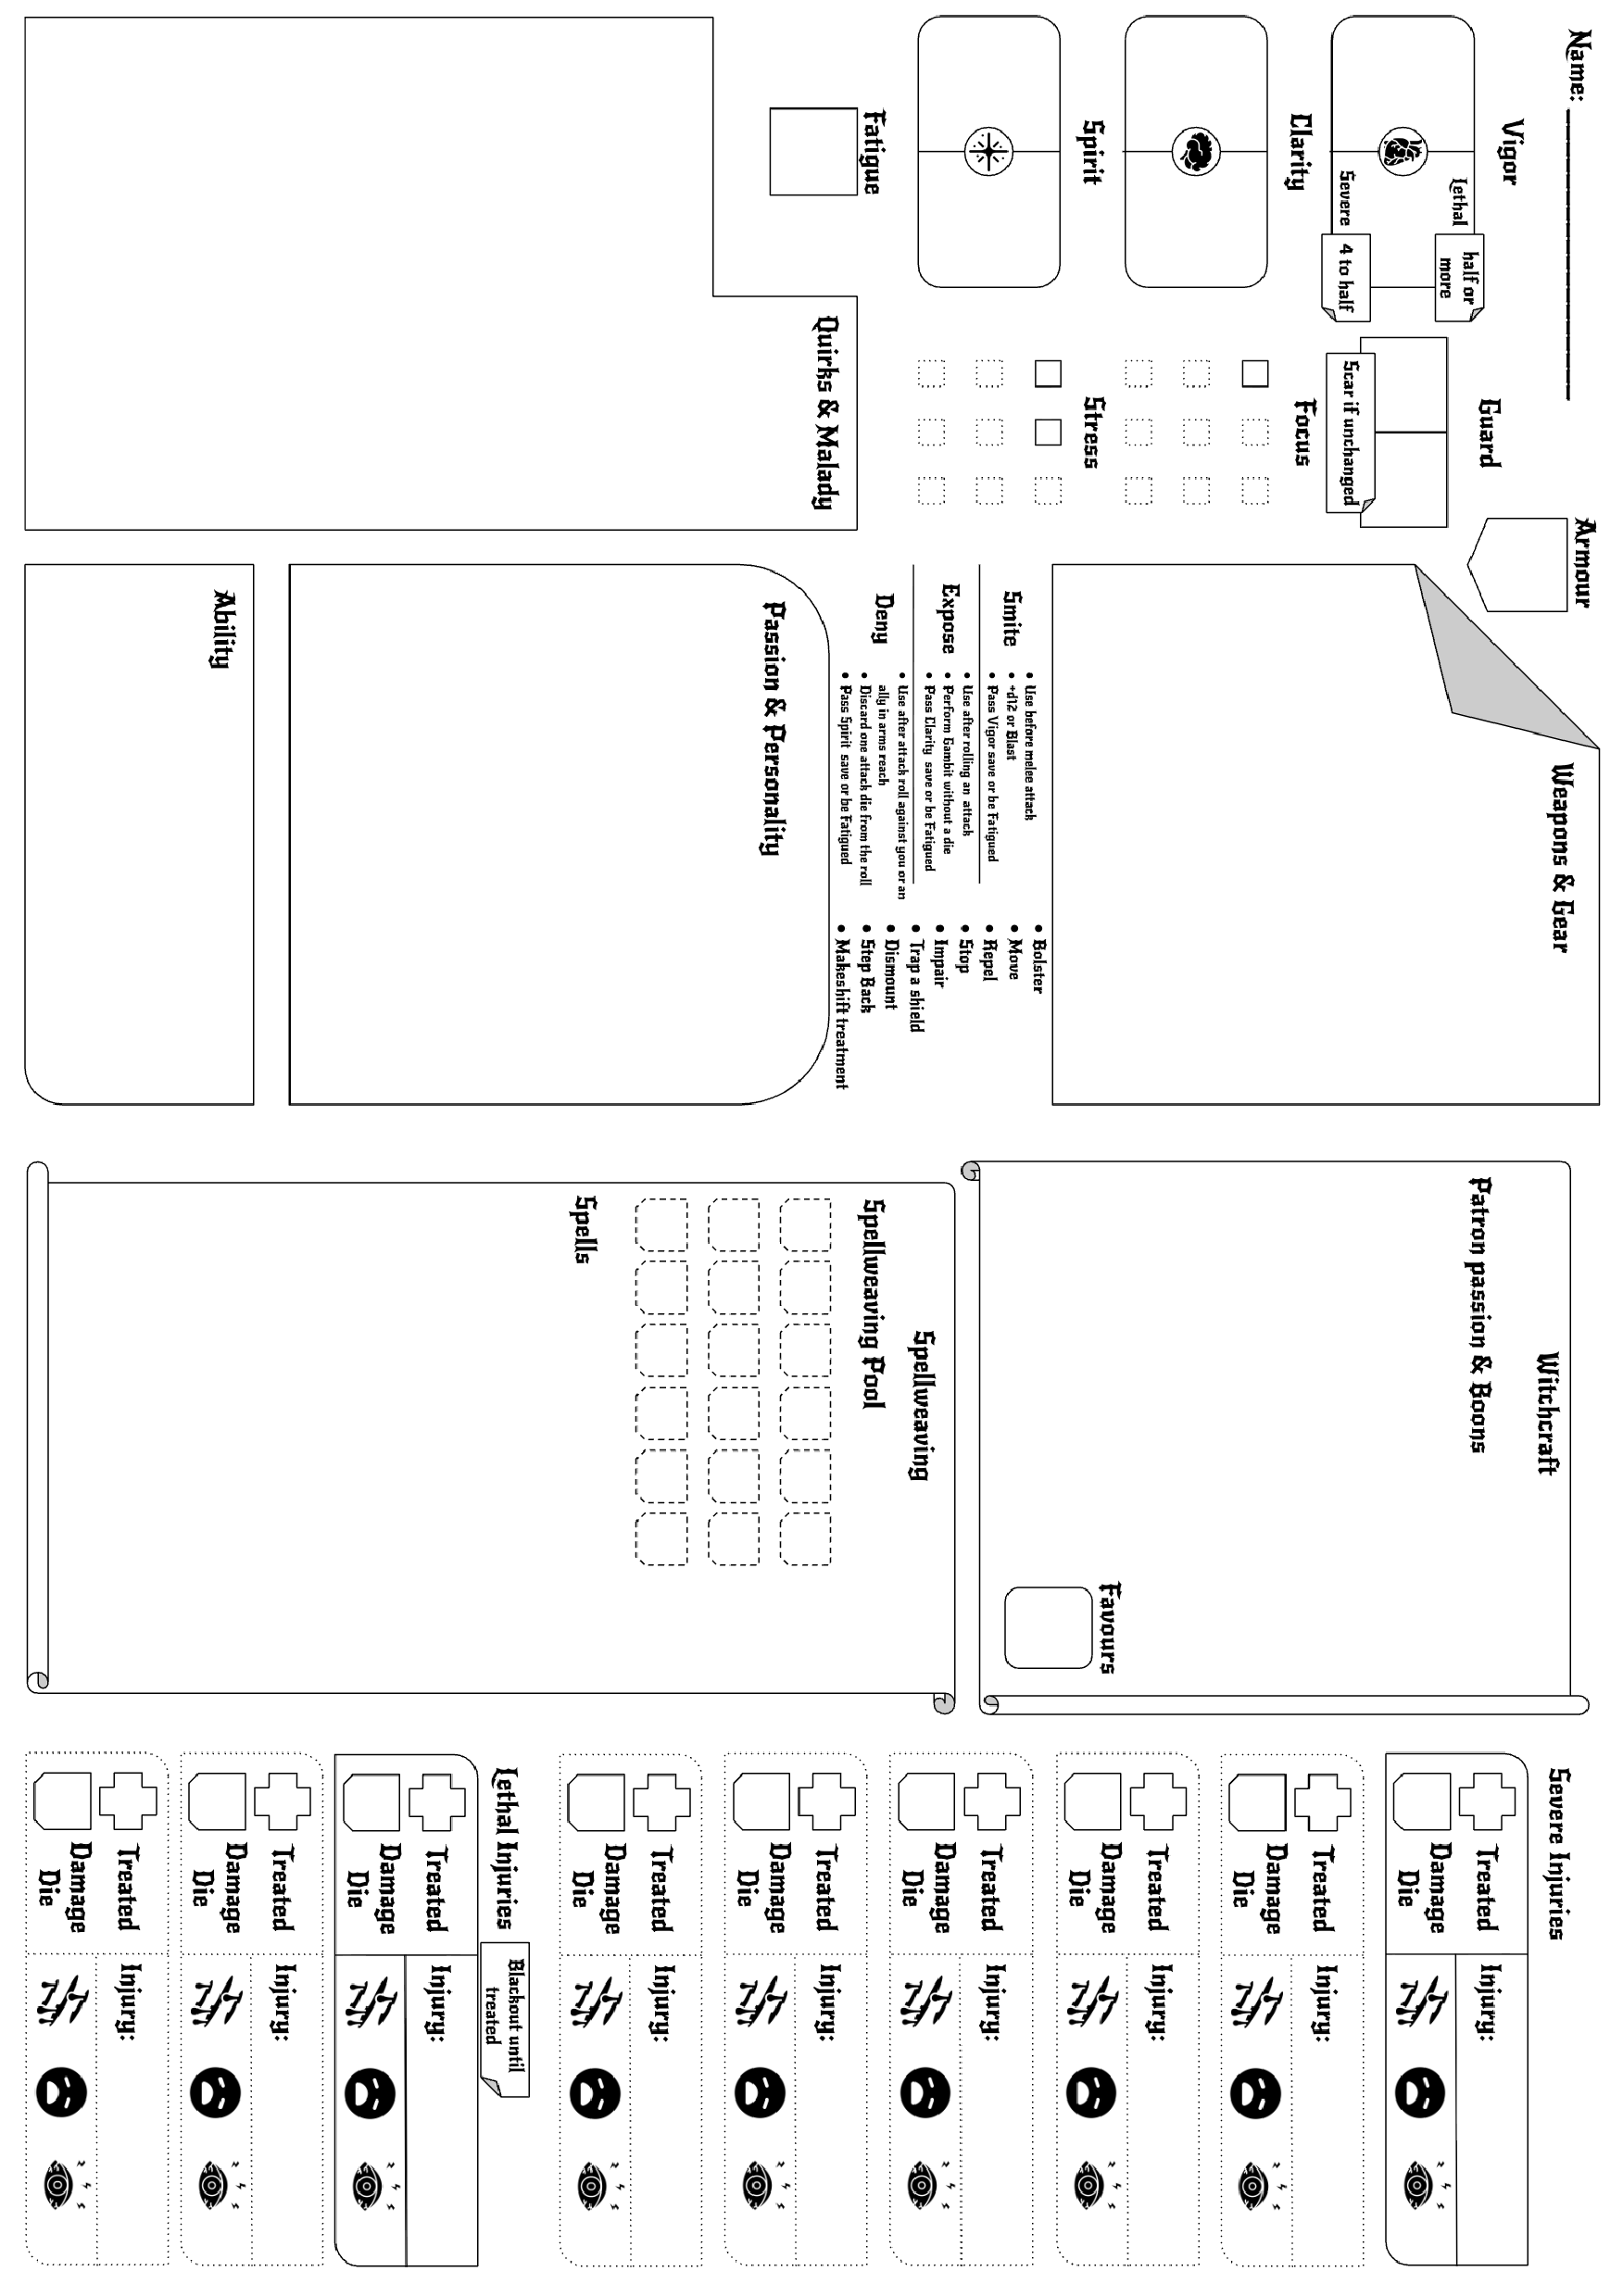
\includepdf[pages={1}]{media/character-sheet.pdf}


\end{document}